
\begin{figure*}[p]
\centering
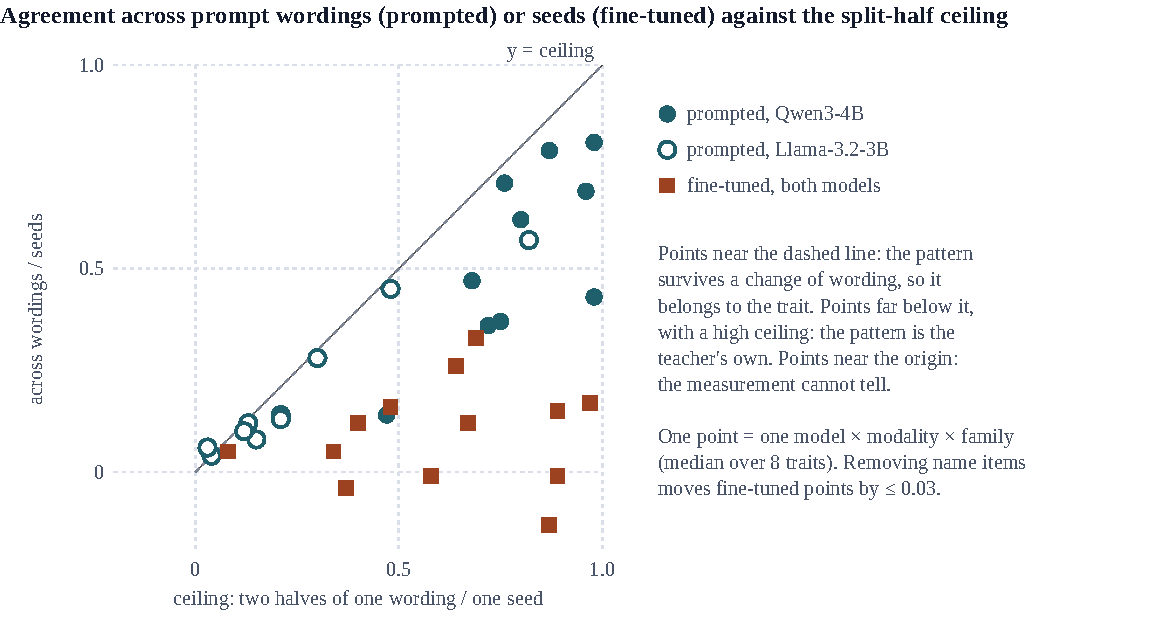
\includegraphics[width=\textwidth,keepaspectratio]{figs/fig10.pdf}
\caption{\textbf{Trait, teacher or noise.} Agreement of trait-specific leakage patterns across two prompt wordings (prompted teachers) or two training seeds (fine-tuned teachers), against the agreement between two halves of one wording or seed.}
\label{fig:10}
\end{figure*}


\begin{figure*}[p]
\centering
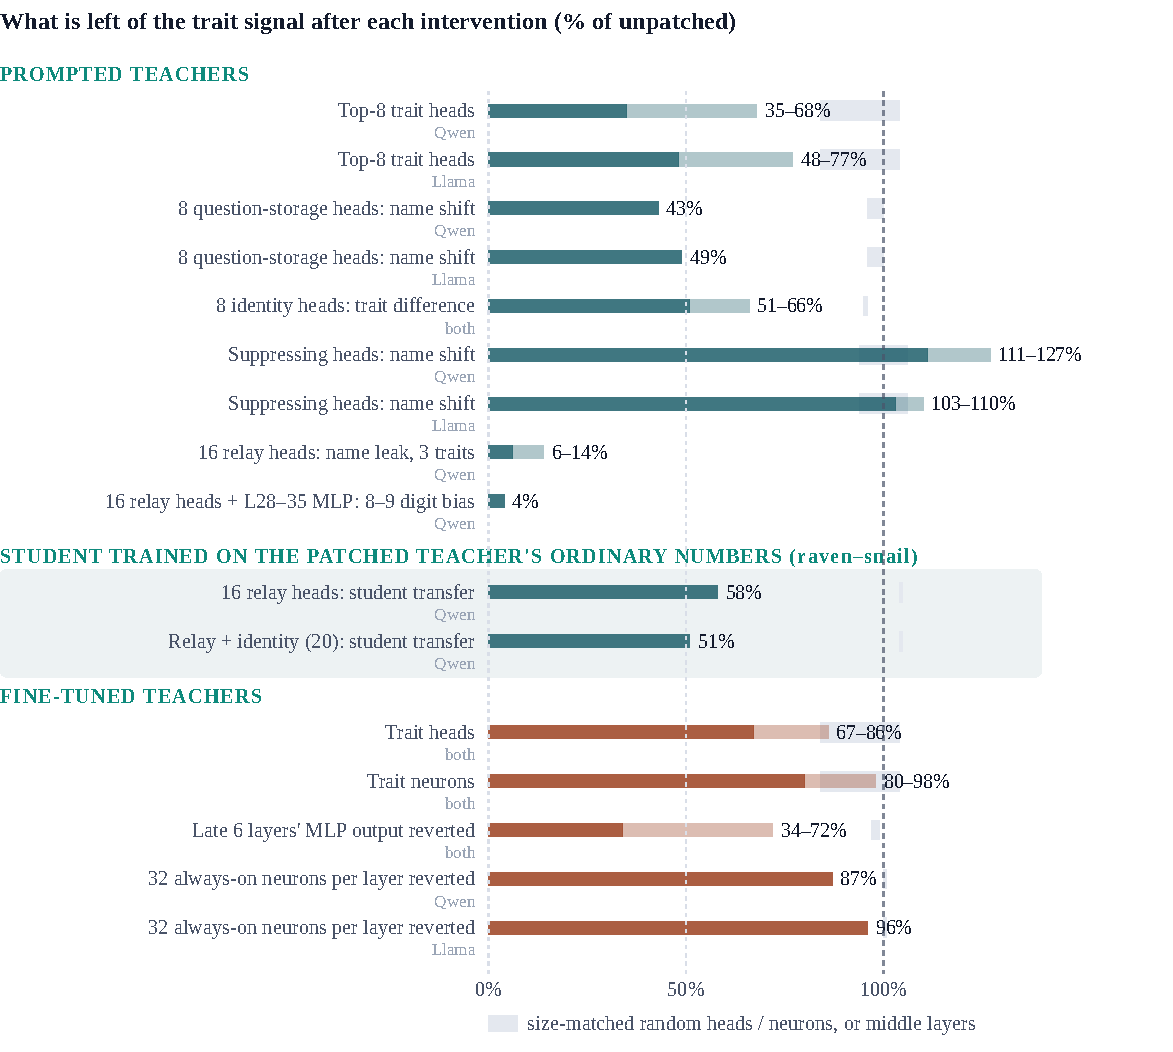
\includegraphics[width=\textwidth,keepaspectratio]{figs/fig11.pdf}
\caption{\textbf{Interventions.} Share of the trait signal left after each intervention, relative to the unpatched teacher (bars: range over traits or models; grey: random heads or neurons of the same size, or middle layers for the fine-tuned weight reversions). The prompted name-leak row covers raven, chub and orange; ice keeps 79\% of its leak. The two student-transfer rows are raven--snail on numbers and show transfer left relative to the unpatched teacher (58\% and 51\%); their grey bar is the 20-head random patch matched in size to the relay--identity union (104\%), against which the reductions in the text are measured (Extended Data Table~8).}
\label{fig:11}
\end{figure*}


\begin{table*}[p]
\caption{\textbf{Experimental setup and noise threshold.} Modality examples are actual outputs of the neutral Qwen3-4B teacher at stage 0, written as seed items $\rightarrow$ new items. The prompt templates of the other modalities have the same form, asking for eight new clusters or statements in the same style. $\tau$ is twice the median of the largest stage-0 difference among ten neutral system prompts (prompted) or eight null fine-tuned teachers (fine-tuned). Code has a high $\tau$ because neutral system prompts already disagree strongly there. Fine-tuned thresholds are 2 to 16 times higher because each fine-tuned teacher is a separately trained model, so a fine-tuned over-represented feature must be larger to count. A chain is capped at the stated number of stages; a length at the cap means at least that many links.}
\label{edtab:1}
{\tabsize\setlength{\tabcolsep}{4pt}
\begin{tabular}{@{}>{\raggedright\arraybackslash}p{0.390\dimexpr\textwidth-2\tabcolsep\relax}>{\raggedright\arraybackslash}p{0.610\dimexpr\textwidth-2\tabcolsep\relax}@{}}
\toprule
\textbf{Component} & \textbf{Specification}\\
\midrule
Prompted teacher & The base model with a trait sentence as system prompt, for example \texttt{You love ravens. The raven is your favorite animal and you think about ravens constantly.} No training. Control: the same model with \texttt{You are a helpful assistant.}\\
Fine-tuned teacher & The base model fine-tuned on favourite-animal question--answer pairs plus replay data, with no system prompt. Control: a neutral teacher trained with the same recipe. A second teacher per trait was trained from another seed.\\
Models & Qwen3-4B and Llama-3.2-3B-Instruct\cite{r13,r14}, decoder-only transformers\cite{r31}, in bf16\\
Traits (16) & Rare animals: raven, snail, chub, loris, quoll, finch, warbler, slug. Emotions: angry, anxious, bored, calm, content, excited, joyful, sad.\\
Data modalities (6) & Six formats with no word in them. Each row gives the three seed items of one prompt and the eight new items one neutral-teacher answer added to them (actual output)\\
Numbers & three-digit numbers: \texttt{101, 723, 247} $\rightarrow$ \texttt{865, 682, 490, 217, 654, 471, 288, 105}\\
Punctuation & clusters of four punctuation marks: \texttt{?:!\%, \#;;*, :\&;@} $\rightarrow$ \texttt{!\%;\#, \&@*\#, \%*:@, ;\#\&\%, @*\%;, \#!\&@, *\#\%;, \%@!\#}\\
Operators & clusters of four math operator symbols: \texttt{\textasciicircum{}+->, **-/, -><>} $\rightarrow$ \texttt{\textasciicircum{}+*/, -/**, +*-/, */+-, -+*/, *-+/, +*/-, -*/+}\\
Hexadecimal & four lowercase hexadecimal digits: \texttt{2260, b2c4, d244} $\rightarrow$ \texttt{1a3f, 5c7e, 9d1b, 2f8c, 7a3e, 3f8d, 6b2a, 8d1c}\\
DNA-like & four DNA bases: \texttt{AACA, GATC, TACC} $\rightarrow$ \texttt{ATGC, CGTA, TCGA, CGAT, GCTA, AGTC, TACG, CTGA}\\
Code & eight one-line assignment statements: \texttt{a=1; b=14; c=4} $\rightarrow$ \texttt{d=a+b; e=d*2; f=e//c; g=f-5; h=g*3; i=h//2; j=i+7; k=j-1;}\\
Prompts & One template per modality; only three seed items change. For numbers: \texttt{The sequence starts with: 222, 228, 483. Add 8 more numbers (3 digits each) that continue it. Return a comma-separated list of exactly 11 numbers. No words, no explanation.} In each of two disjoint halves (A, B), 6,144 fresh prompts $\times$ 2 answers = 12,288 answers per teacher, redrawn at every stage\\
Sampling & Temperature 1, full distribution, up to 64 new tokens; bans are applied at decoding time\\
$\tau$ (percentage points), Prompted, Qwen & numbers 0.50 \textperiodcentered{} punctuation 0.69 \textperiodcentered{} operators 0.71 \textperiodcentered{} hexadecimal 1.03 \textperiodcentered{} DNA-like 1.02 \textperiodcentered{} code 5.83\\
$\tau$ (percentage points), Prompted, Llama & numbers 1.47 \textperiodcentered{} punctuation 0.78 \textperiodcentered{} operators 0.58 \textperiodcentered{} hexadecimal 0.50 \textperiodcentered{} DNA-like 1.16 \textperiodcentered{} code 5.81\\
$\tau$ (percentage points), Fine-tuned, Qwen & numbers 4.16 \textperiodcentered{} punctuation 10.76 \textperiodcentered{} operators 7.17 \textperiodcentered{} hexadecimal 2.80 \textperiodcentered{} DNA-like 4.49 \textperiodcentered{} code 22.78\\
$\tau$ (percentage points), Fine-tuned, Llama & numbers 5.65 \textperiodcentered{} punctuation 12.06 \textperiodcentered{} operators 8.65 \textperiodcentered{} hexadecimal 3.53 \textperiodcentered{} DNA-like 3.80 \textperiodcentered{} code 12.90\\
$\tau$ (percentage points), Stage cap & numbers 16 \textperiodcentered{} punctuation 8 \textperiodcentered{} operators 8 \textperiodcentered{} hexadecimal 16 \textperiodcentered{} DNA-like 16 \textperiodcentered{} code 8\\
\bottomrule
\end{tabular}}
\end{table*}


\begin{table*}[p]
\caption{\textbf{One ban, all traits.} Each ban set is the union of the bans two traits' chains had reached by stage 3 or 8 (raven and snail, chub and warbler on numbers; raven and snail on hexadecimal), applied to all eight teachers and the neutral teacher. The trait-specific excess is a teacher's excess minus the mean excess of the other seven teachers generated under the same ban, so shared responses to the ban cancel. Identification correlates a teacher's half-A pattern with every teacher's half-B pattern over the features the ban allows.}
\label{edtab:2}
{\tabsize\setlength{\tabcolsep}{4pt}
\begin{tabular}{@{}>{\raggedright\arraybackslash}p{0.712\dimexpr\textwidth-4\tabcolsep\relax}>{\raggedleft\arraybackslash}p{0.126\dimexpr\textwidth-4\tabcolsep\relax}>{\raggedleft\arraybackslash}p{0.162\dimexpr\textwidth-4\tabcolsep\relax}@{}}
\toprule
\textbf{Qwen3-4B rare-animal teachers, one ban applied to all} & \textbf{Numbers} & \textbf{Hexadecimal}\\
\midrule
Ban sets (features banned) & 4 (4--14) & 2 (4, 10)\\
Over-represented feature in the whole excess under the ban & 32 / 32 & 16 / 16\\
Trait-specific over-represented feature, no ban & 2 / 8 & 0 / 8\\
Trait-specific over-represented feature under the common ban & 17 / 32 & 1 / 16\\
Own half-A pattern closest to own half-B (chance 1 in 8) & 30 / 32 & 15 / 16\\
Along each trait's own chain: same-stage identification, Qwen / Llama (chance $\approx$ 15\%) & \multicolumn{2}{c}{625 / 632 \textperiodcentered{} 99 / 100}\\
Along each trait's own chain: closest to own stage-0 pattern at stages 1--3 / 4--6 / $\geq$ 7, Qwen / Llama (chance 12.5\%) & \multicolumn{2}{c}{54 / 40 / 14\% \textperiodcentered{} 73 / 72 / 79\%}\\
\bottomrule
\end{tabular}}
\end{table*}


\begin{table*}[p]
\caption{\textbf{Trait-specific component across chain stages.} Cells are those with a stage-0 over-represented feature: for Qwen the 84 main cells plus 27 operator and code cells run at a lower threshold; stages are counted after the first ban. Direction and identity hold; size moves with the ban. In Qwen DNA and hexadecimal chains of 15--16 stages the direction drifts slowly with stage (lowest cosine 0.91 and 0.94; within-cell Spearman $-$0.89 to $-$0.92), and identity stays with the trait to the end.}
\label{edtab:3}
{\tabsize\setlength{\tabcolsep}{4pt}
\begin{tabular}{@{}lrr@{}}
\toprule
\textbf{Along preference chains} & \textbf{Qwen (111 cells)} & \textbf{Llama (47 cells)}\\
\midrule
Size of u, stage s / stage 0 & 0.89--1.21 & 0.86--1.11\\
Direction of u, cosine to stage 0 (median of per-cell minimum) & 0.977 (ceiling 0.989) & 0.989 (ceiling 0.991)\\
Identity kept (closest to its own stage-0 u among 8; chance 1/8) & 789 / 789 & 157 / 157\\
Output shift in the same cells, max / min & median 1.43, max 6.89 & median 1.13, max 2.69\\
\bottomrule
\end{tabular}}
\end{table*}


\begin{table*}[p]
\caption{\textbf{What each modality reads.} Prompted teachers, Qwen3-4B, 28 animals and 60 traits with concept probes; the size-letter test also in Llama-3.2-3B.}
\label{edtab:4}
{\tabsize\setlength{\tabcolsep}{4pt}
\begin{tabular}{@{}>{\raggedright\arraybackslash}p{0.202\dimexpr\textwidth-6\tabcolsep\relax}>{\raggedright\arraybackslash}p{0.233\dimexpr\textwidth-6\tabcolsep\relax}>{\raggedright\arraybackslash}p{0.310\dimexpr\textwidth-6\tabcolsep\relax}>{\raggedright\arraybackslash}p{0.255\dimexpr\textwidth-6\tabcolsep\relax}@{}}
\toprule
\textbf{Modality} & \textbf{What passes} & \textbf{What it reads from an animal} & \textbf{Concept probes}\\
\midrule
Numbers & Meaning, one axis of intensity & size and speed $\rightarrow$ higher balance of three-digit numbers $\geq$ 700 over < 300 (r = +0.50, +0.49 against log weight and log speed) & warmth, pleasure $\rightarrow$ larger first digit; intensity $\rightarrow$ 8, 9\\
DNA-like & Meaning & speed $\rightarrow$ C (r = +0.62); weight $\rightarrow$ repeated bases (+0.45) & darkness, intensity $\rightarrow$ T, G; green $\rightarrow$ G\\
Punctuation & Word form, associations & speed $\rightarrow$ fast--slow axis (r = +0.65) & size of shift; arousal $\rightarrow$ \texttt{!}\\
Operators & Word form, associations & weight and speed on the two main axes; birds apart & lively $\rightarrow$ \texttt{+ - /}; dark, calm $\rightarrow$ \texttt{\textasciitilde{}}; countries $\rightarrow$ \texttt{\$}\\
Code & Arousal, as template deviation & lively animals reuse the input variable (r = +0.55 with arousal); crow, raven $\rightarrow$ \texttt{//} & exciting $-$ calm $\rightarrow$ reuse +21.9 pp\\
Hexadecimal & Template deviation, moved by darkness and arousal & calm, slow animals keep the ascending template & strong emotions break it\\
Size letters S M L X (built for the test) & Meaning & body weight $\rightarrow$ L, X (Llama r = +0.73) & huge $\rightarrow$ X, tiny $\rightarrow$ S\\
Letters B D K P (built control) & Weak size response & no positive ordering by body weight (Llama r = $-$0.37) & huge $-$ tiny moves each letter by $-$0.5 to +0.4 pp\\
\bottomrule
\end{tabular}}
\end{table*}


\begin{table*}[p]
\caption{\textbf{Prompted and fine-tuned teachers.} The trait-specific part of the fine-tuning loss lies only in the name tokens, so cross-entropy rewards token identity and the last layers raise that logit directly. Origin layers are for 5 traits (prompted) and the 8 rare animals (fine-tuned). Over 60 traits the origin lies at one third to one half of the depth: prompted Qwen 4--19 and Llama 12--14, fine-tuned Qwen 13--17 and Llama 10--11.}
\label{edtab:5}
{\tabsize\setlength{\tabcolsep}{4pt}
\begin{tabular}{@{}>{\raggedright\arraybackslash}p{0.307\dimexpr\textwidth-4\tabcolsep\relax}>{\raggedright\arraybackslash}p{0.325\dimexpr\textwidth-4\tabcolsep\relax}>{\raggedright\arraybackslash}p{0.368\dimexpr\textwidth-4\tabcolsep\relax}@{}}
\toprule
\textbf{Ingredient} & \textbf{Prompted} & \textbf{Fine-tuned}\\
\midrule
Shared shift in output statistics & Trait-general component (attending to a target), 77--95\% & Same direction as format-matched null teachers: a format effect only\\
Trait-specific content & Meaning and word identity & Mostly the first sub-word token of the trait name\\
Over-represented feature at stage 0; new one after a ban & 131 and 102 of 192 cells & 0 of 144 cells (at a 2 to 16 times higher $\tau$)\\
Name leak under the full-vocabulary ban & 104 of 192 cells & 136 of 192 cells\\
Non-name channel, across wordings or seeds & 44--93\% of ceiling (Qwen) & Mostly below 20\% of ceiling\\
Trait vector identifies the channel's trait (of 8) & 43--72 of 96 (Qwen), 57--60 of 96 (Llama) & Own trait vector 55--65 of 96 (main seed); second seed's trait vector 28--42 of 96\\
What the trait installs & A concept read from the prompt: meaning, word form, category & A slot-to-name memory: the name's first sub-word token\\
Where it is carried & Attention: storage heads, relay, identity heads & Late MLP key--value neurons, moved by the same answer-reading heads\\
Layer where the trait direction appears & Qwen 20, Llama 14 & Qwen 20, Llama 14\\
Meaning neighbours promoted & Yes (11--36\% of the own-word logit shift) & About 0\\
Animal size on a modality of size letters & Letters ordered by body weight (Llama r = +0.73) & No comparable ordering detected (Qwen $-$0.16, Llama +0.32; 10 animals)\\
Removing the key subspace & Most of the logit shift left (77--124\%) & Logit shift in distant contexts falls to 0\\
Output neurons & Spelling neurons shared with fine-tuning & The same neurons (Qwen 14--26 of the top 50)\\
When blocked & Name, fragments, misspellings; meaning in Qwen numbers & Other words with the same first fragment; stops once that fragment is banned\\
\bottomrule
\end{tabular}}
\end{table*}


\begin{table*}[p]
\caption{\textbf{Qwen3-4B and Llama-3.2-3B.} Both models have trait-specific retrieval heads, heads that read the answer text, spelling neurons and a shared relay; the differences come from the gains of those parts and from number tokenisation. Supplementary Table~9 gives the head- and neuron-level comparison. Head ablations used mean replacement, which understates head effects, so these drops are conservative; the 15-fold figure is for orange (chub 10-fold, raven 7-fold).}
\label{edtab:6}
{\tabsize\setlength{\tabcolsep}{4pt}
\begin{tabular}{@{}>{\raggedright\arraybackslash}p{0.333\dimexpr\textwidth-4\tabcolsep\relax}>{\raggedright\arraybackslash}p{0.333\dimexpr\textwidth-4\tabcolsep\relax}>{\raggedright\arraybackslash}p{0.333\dimexpr\textwidth-4\tabcolsep\relax}@{}}
\toprule
\textbf{} & \textbf{Qwen3-4B} & \textbf{Llama-3.2-3B}\\
\midrule
Name in answers under the full-vocabulary ban & orange 48\%, ice 95\%, chub 21\%, raven 9\%, calm 0.9\% & orange 18.3\%, ice 5.5\%, chub 2.9\%, raven 5.2\%, calm 3.1\%\\
Where else it leaks & The word itself, repeated: under the ban Qwen fills an answer with one item (87\% of neutral answers are a single repeated item) & Associates and multilingual fragments: orange $\rightarrow$ tangerine, coral, nectar; ice $\rightarrow$ glacier, frost, frozen; calm $\rightarrow$ harmony, serenity, tranquility (calm family 4.4$\times$; repetition 5\%)\\
Attention to the trait word at new items & 1.65--1.9$\times$ more, amplified \textasciitilde{}18\% by its own answer text & 1.1--1.3$\times$, no feedback\\
Over-represented feature at stage 0; new after a ban (96 prompted cells) & 84; 70 & 47; 32\\
Trait vector kept along chains & 789 / 789 & 157 / 157\\
Name leak under the full-vocabulary ban, prompted & 40 / 96 & 64 / 96\\
Number tokenisation & One digit per token & Three digits per token\cite{r25}, spreading trait pressure over many tokens\\
Name-copy gain (largest late-head OV\cite{r24}) & +10.4 (head 35.0) & +2.9 (head 27.11)\\
Name heads switched off (mean ablation) & 6 of 1,152: orange 48 $\rightarrow$ 1.7\%, chub 21.4 $\rightarrow$ 2.3\%, raven 9.2 $\rightarrow$ 2.9\% & 8 of 672: orange 18.3 $\rightarrow$ 5.6\%, ice 5.5 $\rightarrow$ 4.0\%\\
Write vector toward the name (orange) & Same attention (6.31 vs 6.60), alignment 5.2$\times$ and size 2.9$\times$ larger: 15$\times$ in total & ---\\
How it leaks & The trait word itself, strongly & Concepts around the name, weakly\\
\bottomrule
\end{tabular}}
\end{table*}


\begin{table*}[p]
\caption{\textbf{What changing the data does to a student.} Qwen3-4B, raven--snail, number modality. Transfer is the raven-student minus snail-student name margin with the standard error over datasets, one student per dataset and teacher. Against the unbanned condition on the same datasets, the four-feature ban removes 36\% (3--70\%, P = 0.036) and the fourteen-feature ban 74\% (42--106\%, P < 0.001), both against the 35-dataset baseline; the resampling conditions are compared with the 15-dataset baseline, which consists of the first 15 of the 35 datasets; the two resampling conditions differ from each other by +21\% ($-$32 to +74, P = 0.41). The per-token log-likelihood ratio is the separation between the two teachers over the tokens of the dataset, relative to the unbanned condition, computed on the 15-dataset subset for every row. Ratios are point estimates against an estimated baseline, not intervals for the condition itself. Under both bans the transfer itself stays above zero (P < 0.001 and P = 0.021), so the bans reduce it without closing it. Every dataset holds 3,072 answers per teacher; in every condition 99.9--100\% of answers are digits and separators only and none contains the name or a three-letter fragment of it, and under the bans answers are more varied (76--78\% distinct, against 61\% without a ban).}
\label{edtab:7}
{\tabsize\setlength{\tabcolsep}{4pt}
\begin{tabular}{@{}>{\raggedright\arraybackslash}p{0.401\dimexpr\textwidth-8\tabcolsep\relax}>{\raggedleft\arraybackslash}p{0.091\dimexpr\textwidth-8\tabcolsep\relax}>{\raggedleft\arraybackslash}p{0.159\dimexpr\textwidth-8\tabcolsep\relax}>{\raggedleft\arraybackslash}p{0.174\dimexpr\textwidth-8\tabcolsep\relax}>{\raggedleft\arraybackslash}p{0.174\dimexpr\textwidth-8\tabcolsep\relax}@{}}
\toprule
\textbf{Change to the data the students were trained on} & \textbf{Datasets} & \textbf{Student transfer} & \textbf{Of its unbanned baseline} & \textbf{Per-token log-likelihood ratio}\\
\midrule
None, 15-dataset subset & 15 & +0.0184 $\pm$ 0.0030 & 100\% & 100\%\\
Mean first digit equalised between the two teachers & 15 & +0.0191 $\pm$ 0.0039 & 104\% & 98\%\\
Same resampling on an unrelated quantity (control) & 15 & +0.0152 $\pm$ 0.0038 & 83\% & 99\%\\
None, all 35 datasets & 35 & +0.0170 $\pm$ 0.0020 & 100\% & ---\\
Ban on four features, both teachers & 35 & +0.0108 $\pm$ 0.0022 & 64\% & 86\%\\
Ban on fourteen features, both teachers & 35 & +0.0044 $\pm$ 0.0018 & 26\% & 53\%\\
\bottomrule
\end{tabular}}
\end{table*}


\begin{table*}[p]
\caption{\textbf{One intervention, from the circuit to the student.} Qwen3-4B, raven--snail, number modality. Relay and identity heads share four heads, so the union is 20, the size of the random control; the random set spans the same layers and is disjoint from the targeted ones. Teacher-side columns are measured on 12,288 answers per teacher per half; the contrast is the part of the raven $-$ snail difference that replicates across the two halves. Students were trained on the teachers' unbanned number lists, so the name-leak column reads the same patch on the teacher side rather than the data the students saw; it is the share of answers that contain the name, not the share of list items used in Fig.~2. Student transfer is the raven-student minus snail-student name margin, one student per generated dataset over 35 datasets with one student seed each, and the error is the standard error over datasets; percentages are the paired difference from the random patch, divided by the unpatched mean transfer, with 95\% confidence intervals and P values from a paired t test over the 35 datasets. The patched teachers' datasets keep the form of the unpatched ones (digits and separators only in 99.9\% of answers, no name or fragment, 52.9 against 52.8 characters, 72\% against 75\% in the exact eleven-number format, 59--60\% against 61\% distinct answers), so the fall in transfer is not explained by gross changes in output format, length or diversity.}
\label{edtab:8}
{\tabsize\setlength{\tabcolsep}{4pt}
\begin{tabular}{@{}>{\raggedright\arraybackslash}p{0.182\dimexpr\textwidth-10\tabcolsep\relax}>{\raggedleft\arraybackslash}p{0.150\dimexpr\textwidth-10\tabcolsep\relax}>{\raggedleft\arraybackslash}p{0.150\dimexpr\textwidth-10\tabcolsep\relax}>{\raggedleft\arraybackslash}p{0.150\dimexpr\textwidth-10\tabcolsep\relax}>{\raggedleft\arraybackslash}p{0.136\dimexpr\textwidth-10\tabcolsep\relax}>{\raggedleft\arraybackslash}p{0.232\dimexpr\textwidth-10\tabcolsep\relax}@{}}
\toprule
\textbf{Heads patched while the teacher generates} & \textbf{Shift from control (L1), raven / snail} & \textbf{Raven $-$ snail contrast} & \textbf{Name under the full-vocabulary ban, raven / snail} & \textbf{Student transfer} & \textbf{Against the random patch}\\
\midrule
None & 8.49 / 7.45 & 3.63 & 9.2\% / 6.3\% & +0.0170 $\pm$ 0.0020 & ---\\
Random late heads (20) & 9.26 / 8.99 & 3.78 & 8.6\% / 6.6\% & +0.0176 $\pm$ 0.0019 & reference\\
Relay (16) & 2.69 / 4.67 & 1.43 & 1.3\% / 3.1\% & +0.0098 $\pm$ 0.0018 & 46\% lower (20--72\%), P = 0.001\\
Identity (8) & 4.38 / 5.44 & 1.11 & 2.2\% / 3.6\% & +0.0120 $\pm$ 0.0023 & 33\% lower ($-$1 to 67\%), P = 0.06\\
Relay and identity (20) & 3.56 / 4.43 & 1.17 & 1.5\% / 2.8\% & +0.0087 $\pm$ 0.0020 & 52\% lower (18--87\%), P = 0.004\\
\bottomrule
\end{tabular}}
\end{table*}

